\documentclass[12pt]{article}
\usepackage{graphicx} % Required for inserting images
\usepackage{listings} % for python code
\usepackage{dirtree} % for directory trees
\usepackage{hyperref} % for hyperlinks

\title{\textbf{Applied Data Analytics} \\
Tackling Data Version Management in MLOps using DVC}
\author{Sampad Kumar Kar(MCS202215) \\
Shourjya Basu(MCS202207) \\
\textbf{Mentor: Dr. M. Chandramouli}}

\date{10th December 2023}
\begin{document}

\maketitle

\tableofcontents

\newpage

\section{Introduction}

MLOps, short for Machine Learning Operations, is a discipline that combines machine learning (ML) and data engineering practices to streamline the end-to-end process of deploying, managing, and monitoring machine learning models in production.

MLOps aims to bridge the gap between data science and IT operations by introducing a set of best practices, tools, and methodologies that enhance collaboration, automation, and reproducibility throughout the machine learning pipeline. This comprehensive approach encompasses various stages, including data preparation, model training, validation, deployment, and ongoing monitoring, ensuring that ML systems are not only accurate during development but also robust and maintainable in real-world environments.

\subsection{Objectives of MLOps}
\begin{itemize}
    \item \textbf{Collaboration}: Implementing tools and practices that facilitate collaboration among data scientists, developers, and other stakeholders, allowing them to work seamlessly on shared projects and contribute to the versioning process.

    \item \textbf{Reproducibility}: Establishing a versioning system that allows the recreation of specific model states, enabling reproducibility of experiments and ensuring consistency across different stages of the machine learning lifecycle.

    \item \textbf{Automation in Machine Learning Pipelines}:DVC can be integrated into machine learning pipelines, including continuous integration and continuous deployment (CI/CD) processes. This enables automated testing and deployment while maintaining the versioning of datasets.
    
    \item \textbf{Scalability}: Addressing the challenges of version management at scale, particularly in environments where multiple models, versions, and iterations coexist, and ensuring that the versioning system remains efficient and effective.
\end{itemize}

\newpage 

\section{Components of MLOps}

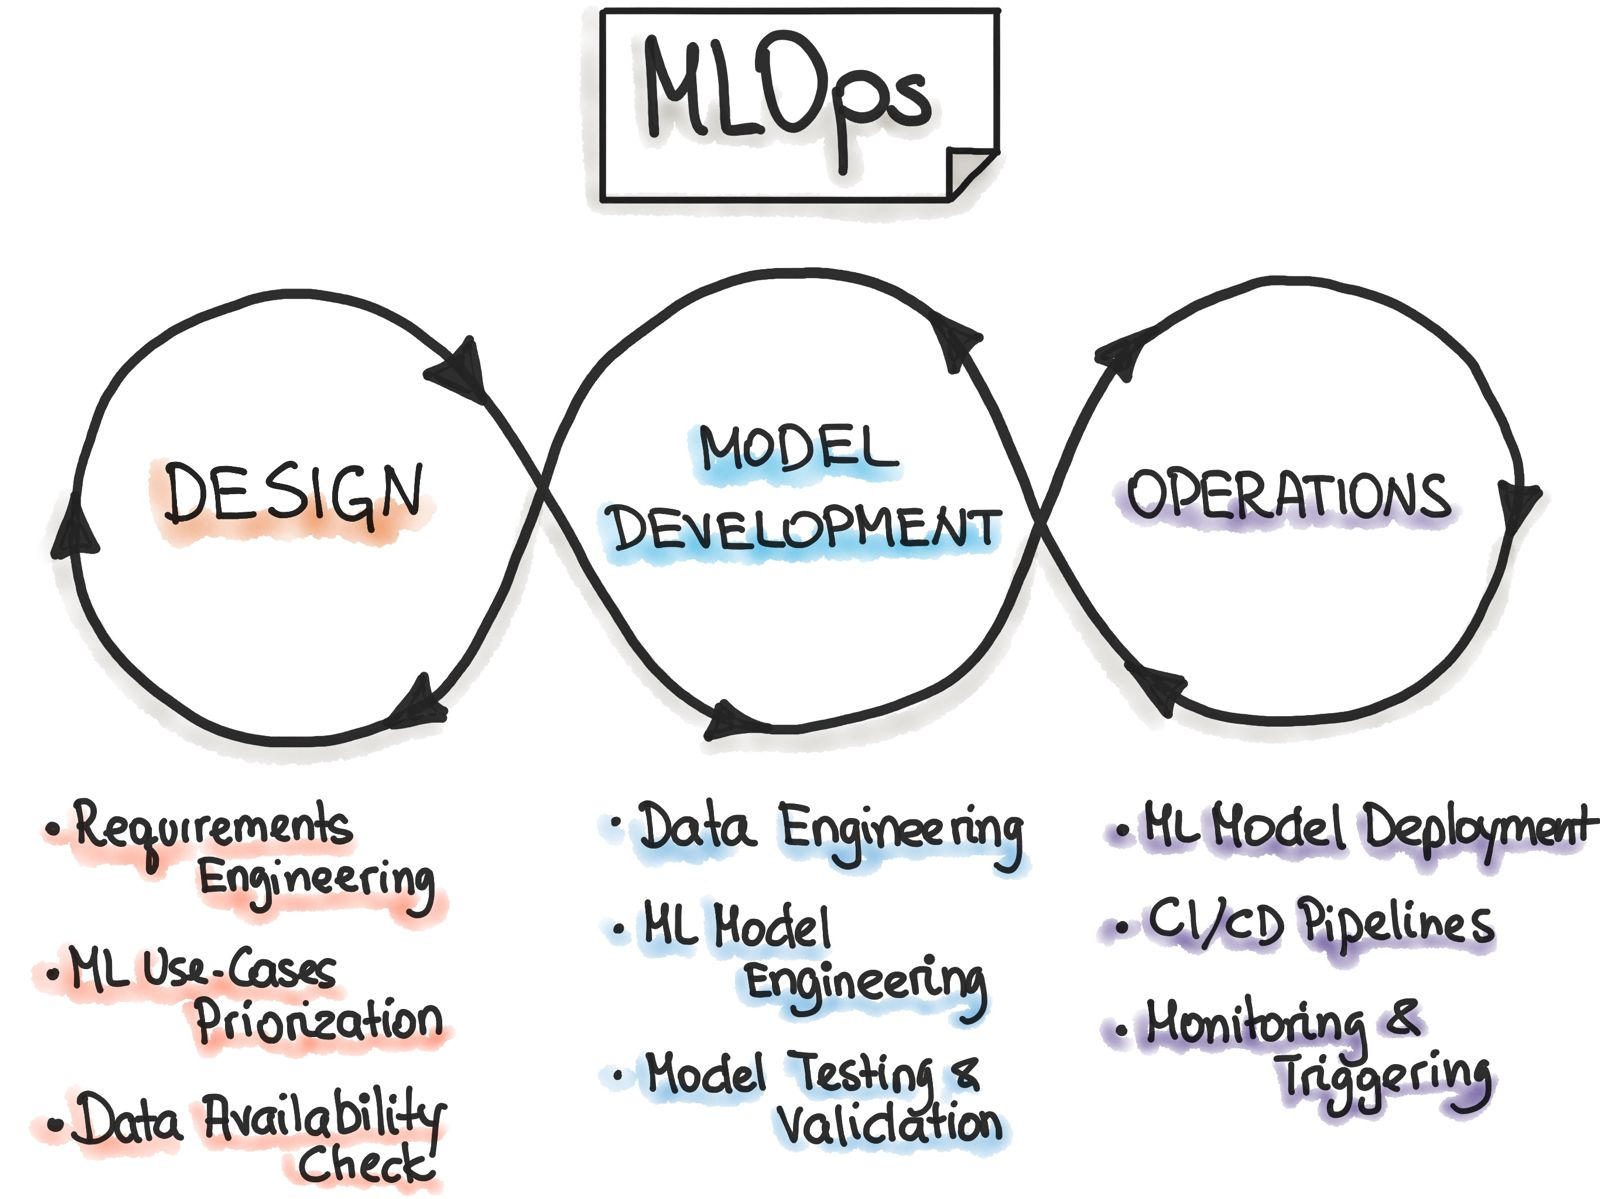
\includegraphics[width = 15cm, height = 10cm]{MLOPS.jpg}

MLOps can be broadly divided into three components.

\subsection{Design}
\begin{itemize}
    \item \textbf{Requirements engineering}: It involves the systematic process of gathering, documenting, and managing the needs and expectations related to machine learning systems. This crucial phase ensures a clear understanding of stakeholders' objectives, business goals, and technical constraints, laying the foundation for the successful development, deployment, and maintenance of machine learning models within an operational environment.

    \item \textbf{ML use-case Prioritization}: It is the process of systematically evaluating and ranking potential machine learning (ML) applications based on their strategic importance, feasibility, and potential impact on business objectives. In the context of ML use-case prioritization, organizations seek to identify and prioritize projects that align with their overall goals, resource constraints, and desired outcomes. This approach helps optimize resource allocation and ensures that ML efforts are focused on initiatives that deliver the greatest value.

    \item \textbf{Data Availability Check}: It is very important that the problem/objective is clearly understood and proper data is considered for the task.
    The design phase aims to inspect the available data that will be needed to train our model and to specify the functional and non-functional requirements of our ML model.
\end{itemize}

\subsection{Model Development}
\begin{itemize}
    \item \textbf{Data Engineering}: Data engineering involves designing, developing, and managing the data architecture, infrastructure, and tools necessary for collecting, storing, processing, and analyzing large volumes of data. It plays a critical role in supporting data-driven decision-making and enabling organizations to derive valuable insights from their data. 

    For example, data should be checked for NULL values, components of data that does not contribute to the problem statement should be losed, it should be checked if any two features of the data are highly correlated, etc.

    \item \textbf{ML Model-Engineering}: ML model engineering refers to the process of designing, developing, and deploying machine learning (ML) models in a systematic and scalable manner. It encompasses a set of practices, principles, and methodologies that focus on the end-to-end lifecycle of machine learning models, from conception and training to deployment and maintenance. ML model engineering aims to address challenges related to reproducibility, scalability, robustness, and collaboration in the development and operationalization of ML models.

    \item \textbf{Model Testing and Validation}: After the model designing is complete, it needs to be tested and validated on test data(data that has not been used for training) before being deployed for public use/business. It is important to make sure that the model works equally well on unseen data as it does on training data. Methods like hyperparameter tuning, cross validation are used to achieve this.
\end{itemize}

\subsection{Operations}
\begin{itemize}
    \item \textbf{ML Model Deployment}: This marks the beginning of the operational phase of the ML model. So far, the ML model was in the development stage and was dealing with previously collected data. It is now deployed to be used in the real world for businesses and problems of various kind. The model comes across the challenges in a real-world scenario.

    \item \textbf{CI/CD Pipelines}: Continuous Integration(CI) is a development practice where developers regularly merge their code changes into a shared repository. The primary goal is to detect and address integration issues early in the development cycle.

    Continuous Deployment(CD) is an extension of CI and involves automatically deploying code changes to production environments after passing the CI tests. 

    By combining CI and CD, development teams can achieve a highly automated and efficient software delivery pipeline. This approach leads to faster feedback, quicker release cycles, and increased overall software quality, ultimately delivering better value to end-users.

    \item \textbf{Monitoring and Triggering}: Monitoring involves the systematic observation and measurement of various aspects of a system, such as its performance, availability, and resource utilization. The goal of monitoring is to gain insights into the system's behavior, detect anomalies or issues, and ensure that it meets predefined performance and reliability criteria.

    Triggering refers to the automatic initiation of actions or processes based on predefined conditions or events. Triggers are often associated with specific events or changes in the system's state, and they can initiate responses such as automated deployments, notifications, or workflow executions.

    In summary, monitoring provides visibility into system behavior, while triggering enables automated responses based on observed conditions. Together, they form a powerful combination for maintaining the reliability, performance, and responsiveness of software systems in dynamic and complex environments.
\end{itemize}
\newpage

\section{Introduction to Version Control}

Version control, also known as source control or revision control, is a system that records changes to a set of files or a codebase over time. It allows multiple contributors to collaboratively work on a project, tracking modifications, and managing different versions of files. Version control systems (VCS) are essential tools in software development and other collaborative projects, providing a structured way to manage changes, resolve conflicts, and maintain a historical record of the project's evolution.

Versionin Control can be used for various purposes:
\begin{itemize}
    \item \textbf{Project Versioning}: It is the practice of systematically managing and tracking changes to a project over time. It involves assigning unique identifiers or version numbers to different states or releases of the project, allowing developers and collaborators to reference and manage specific points in the project's evolution.
    
    \item \textbf{Data Versioning}: It refers to the practice of systematically managing and tracking changes to datasets over time. It is an essential aspect of data management in various fields, including data science, machine learning, and analytics. Data versioning is crucial for maintaining a clear and organized history of dataset changes, facilitating collaboration among data practitioners, ensuring reproducibility, and supporting the development and deployment of machine learning models.
    
    \item \textbf{Model Versioning}: It refers to the systematic management and tracking of changes to machine learning models over time. It involves assigning unique identifiers or version numbers to different iterations or releases of a model, allowing data scientists, engineers, and other stakeholders to reference specific versions and understand the evolution of the model. Model versioning is crucial for reproducibility, collaboration, and effective model lifecycle management.
    
    \item \textbf{Deployment-based Versioning}: It refers to the practice of assigning unique version identifiers to software releases that are deployed to different environments or stages of the development lifecycle. This type of versioning is particularly relevant in scenarios where the model undergoes multiple deployments, such as moving from a development or testing environment to staging, and finally to a production environment.
\end{itemize}

\newpage

\section{Key aspects of Data Versioning}
\begin{itemize}
    \item \textbf{Dataset Versioning}: Similar to code or project versioning, data versioning involves assigning unique identifiers or version numbers to different states or versions of a dataset. This allows data practitioners to reference specific versions of the data and track changes over time.

    \item \textbf{Change Tracking}: Data versioning systems keep track of changes made to a dataset, including additions, modifications, and deletions. This change tracking is valuable for understanding the evolution of the data and identifying the impact of specific modifications.

    \item \textbf{Data Lineage}: Data lineage refers to the ability to trace the origin, transformation, and movement of data throughout its lifecycle. Data versioning contributes to data lineage by documenting changes and relationships between different versions of a dataset.

    \item \textbf{Collaboration}: In collaborative data science or machine learning projects, multiple team members may contribute to dataset preparation and feature engineering. Data versioning allows team members to work on different versions of a dataset concurrently, promoting collaboration without conflicts.

    \item \textbf{Reproducibility}: Reproducibility is a key principle in data science and machine learning. Data versioning ensures that the state of the dataset used for training a model is well-documented, enabling others to reproduce experiments and results.

    \item \textbf{Data Quality Monitoring}: By tracking changes to datasets, data versioning systems can contribute to data quality monitoring. Sudden changes or anomalies in dataset versions may indicate data quality issues that need investigation.

    \item \textbf{Backup and Recovery}: Data versioning serves as a form of backup, allowing organizations to roll back to previous versions in case of errors, data corruption, or unexpected issues.
\end{itemize}

Effective data versioning practices contribute to a more organized and collaborative data environment, supporting the end-to-end data lifecycle from data exploration and preparation to model development and deployment.

\newpage

\section{Research Questions}

In order to comprehensively address the challenges associated with data version management in MLOps, we formulated the following research questions:

\begin{itemize}
    \item \textbf{Current State of Data Versioning in the Marketplace:}
    \begin{itemize}
        \item What is the existing landscape of data versioning tools and practices in the current marketplace within the domain of MLOps?
        \item How do various organizations and practitioners currently address data versioning challenges, and what tools are commonly employed in the industry?
    \end{itemize}

    \item \textbf{Requirements for Implementing Data Versioning in Project Pipelines:}
    \begin{itemize}
        \item What are the essential requirements that must be taken into consideration when integrating data versioning into the project pipeline, particularly in the context of MLOps?
        \item How do these requirements vary across different types of ML projects, and what factors influence the decision-making process for selecting a data versioning solution?
    \end{itemize}

    \item \textbf{Approaches and Frameworks for Integrated ML Systems in Production:}
    \begin{itemize}
        \item What approaches and frameworks are available for building an integrated ML system that can be seamlessly operated in production environments?
        \item How can these approaches be continuously applied to ensure the robust and efficient operation of ML systems over time, and what considerations need to be taken into account for successful implementation?
    \end{itemize}
\end{itemize}

These should provide a comprehensive understanding of the current state of data versioning, the specific requirements for implementing it in MLOps projects, and the available approaches and frameworks for building and maintaining integrated ML systems in production. The answers to these questions will contribute valuable insights to the overall objectives of the project, which aims to leverage DVC for effective data version management in MLOps.

\newpage

\section{Data Versioning Tools: DVC}

DVC is an Open-source, Git-based data science library, developed by iterative.ai, which enables users to apply version control to machine development by tracking ML Models and Data sets. It provides $3$ main functions:

\begin{itemize}
    \item \textbf{ML Project Version Control:} This allows to version control ML Models, datasets and intermediate files. DVC connects them with code, and supports state of the art frameworks like Amazon S3, Microsoft Azure Blob Storage, Google Drive, Google Cloud Storage etc to store the file contents.

    Full code and data provenance help track the complete evolution of every ML model. This guarantees reproducibility and makes it easy to switch back and forth between experiments.

    \item \textbf{ML Experiment Management:} This also allows to harness the full power of Git branches to try different ideas instead of sloppy file suffixes and comments in code. This also allow the use automatic metric-tracking to navigate instead of doing it manually.
    
    \item \textbf{Deployment and Collaboration:} This also simplifies collaboration by the use of push/pull commands to move consistent bundles of ML models, data, and code into production to remote machines or a colleague's computer instead of relying on ad-hock scripts, which could very well go wrong and make it harder to diagnose bugs.
\end{itemize}

Overall, this serves as a comprehensive solution for data versioning in MLOps, which helps align our project with the overarching goal of achieving effective data version management, ensuring reproducibility, and enhancing collaboration in the machine learning development lifecycle.

\newpage

\section{Demo Problem}

In this section, we describe the demo problem that we use to demonstrate the efficacy of DVC as a tool in the general lifecycle of a ML project. The problem titled "Changing Dataset by Modifying Random Seed" is a toy problem which can showcase the capabilities of DVC in the lifecycle of a ML project. The objective is to create a simple classification model using a fixed random seed for the train-test-split step and subsequently modify the random seed to observe the impact of model performance of the newly split data, while we keep track of these changes via DVC. Here are the key steps involved:

\begin{itemize}
    \item \textbf{Creating a Simple Classification Model:} Initiate the process by building a basic classification model, incorporating a random seed for the train-test split. This step is essential for establishing a baseline model using a specific dataset.
    \item \textbf{Modifying the Random Seed:} Alter the random seed used in the train-test split to induce changes in the dataset. This modification simulates a scenario where the dataset undergoes variations, reflecting the real-world dynamics of data evolution in machine learning projects.
    \item \textbf{Observing Impact on Model Performance:} Assess the impact of modifying the random seed on the model's performance. This step provides insights into how changes in the dataset affect the model's predictive capabilities, emphasizing the importance of tracking these alterations for reproducibility and model evaluation.
    \item \textbf{Tracking Changes with DVC and Git:} Utilize DVC in conjunction with Git to systematically track changes to both the dataset and the model. By versioning the data and code, DVC enables the preservation of experiment provenance, ensuring a comprehensive record of alterations made during the development process.
\end{itemize}

We now discuss the specifics related to the Data Versioning aspect of the project, where we describe how DVC and Git function in tandem to allow us to track changes in the data.

\newpage

\subsection{Data Versioning: DVC Implementation}

For version control of ML projects, we need to consider not only the code, but also the data and ML model (i.e. ML artefacts). The following are the steps involved:

\subsubsection{Initialise Git and DVC}
\begin{lstlisting}[language=Python]
    # initialise Git and DVC
    ! git init
    ! dvc init
\end{lstlisting}

DVC is an easy to use tool that works on top of Git. We first intall DVC and initialise it in our project along with Git.

\subsubsection{Versioning ML Artefacts}
Here is the basic file and folder structure of our project:

\medskip

\dirtree{%
.1 /.
.2 data.
.3 raw.
.3 test.csv.
.3 train.csv.
.3 val.csv.
.2 database.
.2 prepare.ipynb.
.2 train.ipynb.
}

\medskip

Here, we are interested in \verb|data| directory, which contains our pre-processed \verb|.csv| files after splitting. DVC uses \verb|*.dvc| files which contain unique md5 hash to link the dataset to the project. DVC stores the copy of this data file into DVC cache, using the first two letters of the hash as the folder name. Here is how the \verb|data| folder looks after we start trakcing the files by DVC:

\medskip

\dirtree{%
.1 data.
.2 raw.
.2 raw.dvc.
.2 test.csv.
.2 test.csv.dvc.
.2 train.csv.
.2 train.csv.dvc.
.2 val.csv.
.2 val.csv.dvc.
}

\medskip
Then use git commit to track these changes. For instance, this is how we track \verb|train.csv|:
\medskip

\begin{lstlisting}[language=Python]
    # start tracking the train.csv using DVC
    ! dvc add data/train.csv
    ! git add data/train.csv.dvc

    ! git commit -m "start tracking train data"
\end{lstlisting}

\subsubsection{Storing Versioned ML Artefacts}

DVC supports various cloud storage that enables us to store our dataset or models in remote cloud storage i.e. Amazon S3, Google Drive etc. In order to do this, first, we need to setup the remote storage using DVC, then upload the ML artefacts to this remote storage. By doing so, we do not need to keep the large dataset in our Git repository, the lightweight, human-readable \verb|*.dvc| file which contains the link to our real dataset will be kept in the Git repository.

\begin{lstlisting}[language=Python]
    # setup remote storage using DVC
    ! ! dvc remote add -d storage gdrive://folder_code
    ! git add .dvc/config
    ! git commit -m "configure remote storage"
\end{lstlisting}

\subsubsection{Retrieving ML Artefacts}

Having DVC-tracked data stored remotely, it can be downloaded to Git repository when needed. As the DVC file stored in Git repository contains the hash to uniquely identify the data and remote information is stored in DVC config, it knows where to find the data on remote storage and download the data to the local project.

\subsubsection{Making changes on Dataset}

When making changes to dataset locally, the DVC add command allows us to track the latest version of the dataset. It will update the md5 hash inside the DVC file and then the new version of dataset has been linked to the project. For this particular problem, we change our dataset by changing the random seed used during train-test-split. We initially track with a random seed of $42$ and later with $420$. For instance, this is how we would track the changes in the training data:
\medskip
\begin{lstlisting}[language=Python]
    # add the new version of data to track
    ! dvc add data/train.csv
    # push the new version to remote storage
    ! dvc push
    # record the stage for the new version
    ! git commit -m "training data updated"
\end{lstlisting}

\subsubsection{Switch between Versions}

When we want to rollback to a certain version of dataset, git checkout will help us checkout a commit or a revision of DVC file, and then using dvc checkout to synchronize data. We do this in the follwing manner:
\medskip
\begin{lstlisting}[language=Python]
    # add the new version of data to track
    ! dvc add data/train.csv
    # push the new version to remote storage
    ! dvc push
    # record the stage for the new version
    ! git commit -m "training data updated"
\end{lstlisting}

\section{Implementation Details}

The codes associated with the demo problem were meticulously recorded in our Git repository, providing a transparent and reproducible record of changes. The repository includes a structured file system illustrating the problem, with key highlights capturing key stages of DVC integration. Here is the link to the repository: \url{https://github.com/sampadk04/Applied_Data_Analytics_Project}

\newpage

\section{Conclusion}

During this project, we aimed to establish a foundational understanding of MLOps and implement version control in a machine learning context using DVC. Our key takeaways underscore the pivotal role of DVC in seamlessly integrating with Git, ensuring reproducibility, and offering a comprehensive solution for tracking changes in datasets and models. The implementation of a demo problem revealed practical insights into the impact of data alterations on model performance, emphasizing the tool's significance in facilitating reliable experiment management.

Amidst our exploration, challenges in managing version control for extensive datasets and complex ML models were encountered, prompting us to balance the need for comprehensive versioning with practical considerations. However, these challenges served as invaluable learning experiences, fostering optimization strategies and enhancing our understanding of efficient data version management. Collaborating as a team and delving into diverse resources broadened our knowledge of industry best practices in MLOps and data versioning, contributing to a holistic learning experience that will undoubtedly inform future ventures in this evolving landscape.

\section{References}
\begin{itemize}
    \item \href{https://repositorio-aberto.up.pt/bitstream/10216/152181/2/636962.pdf}{Tackling Version Management and Reproducibility in MLOps}
    \item \href{https://mcis.cs.queensu.ca/publications/2021/saner.pdf}{On the Co-evolution of ML Pipelines and Source Code}
    \item \href{https://medium.com/y-data-stories/creating-reproducible-data-science-workflows-with-dvc-3bf058e9797b}{Creating reproducible data science workflows with DVC}
    \item \href{https://www.microsoft.com/en-us/research/uploads/prod/2019/03/amershi-icse-2019_Software_Engineering_for_Machine_Learning.pdf}{Software Engineering for Machine Learning: A Case Study}
    \item \href{https://www.mdpi.com/2076-3417/11/19/8861}{Demystifying MLOps and Presenting a Recipe for the Selection of Open-Source Tools}
    \item \href{https://dvc.org}{Official DVC Website}
\end{itemize}
       
\end{document}
